\chapter{ \textit{Big Data}, données biomédicales et \textit{machine-learning}}

Hiding within those mounds of data is knowledge that could change the life of a patient, or change the world
- Atul Butte, 2012

L'informatisation du monde a permis la production et l'accumulation de données de façon exponentielle. En particulier dans le domaine de la santé, les avancées technologiques comme les technologies de séquençage, d'imagerie ou les dossiers médicaux électroniques ont permis au cours du temps la capture de données précieuses pouvant améliorer le parcours et la prise en charge des patients.

Dans le même temps, les technologies d'analyse de données massives (\textit{Big Data}) se sont développées notamment grâce au \gls{ml}, une branche de l'\gls{ia} permettant à des algorithmes informatiques d'apprendre à partir des données. Cette massification des données biomédicales et le développement des technologies d'analyse de données permettent d'entrevoir un monde où les soins de santé pourraient être personnalisés, préventifs et prédictifs .

Dans ce premier chapitre d'introduction, nous présenterons d'abord ce que sont les Big Data, la variété des données biomédicales et comment ces données sont utile pour une meilleure prise en charge des patients. Puis, dans une seconde partie, nous présenterons les concepts principaux du \gls{ml} pour le traitement de ces données.

\section{Les données biomédicales: des \textit{Big Data} au service des patients}

\subsection{Définition du \textit{Big Data}}

Le terme "Big Data" est utilisé pour faire référence à l'immense quantité de données complexes et hétérogènes produites par cette informatisation du monde et le développement des technologies haut débit (\cite{de_mauro_formal_2016}). La définition des Big Data a été enrichie au fur et à mesure des années d'abord par 3 mots clés puis 5 et même jusqu'à 7 (\cite{garcia_what_2022}). La définition la plus commune aujourd'hui des Big Data se compose des 5 "V": le volume, la variété, la vélocité, la véracité et la valeur (\cite{ishwarappa_brief_2015}). Ainsi pour être considérée comme Big Data, les données doivent: (i) être volumineuse, du gigaoctet à l'exaoctet (ii) être variée, c'est-à-dire multimodales (iii) avoir une vélocité de création et de traitement importante (iv) être vérace, c'est-à-dire valide et (v) avoir une forte valeur ajoutée, c'est-à-dire qu'elles doivent être utiles. (\cite{garcia_what_2022}).

Ainsi les données biomédicales sont en adéquation à cette définition (\cite{zheng_application_2021}). Grâce aux améliorations en techniques d'acquisitions (séquençage, imagerie) elles sont volumineuses et possèdent une forte vélocité. Ces données sont variées, contenant des informations sur le plan génétique, phénotypique et histologique. De plus elles ont une véracité assurée couplée à une forte valeur ajoutée. En effet, ce sont de manière générale des données générées par des experts (médecin ou biologiste) et liées à des patients (et donc fortement valorisées). Il est alors juste de parler de qualifier les données biomédicales de Big Data (\cite{sonawane_network_2019}. Ainsi dans la prochaine section nous allons voir en détail les différentes modalités de données biomédicales de patients, leurs acquisitions et les challenges que présente leur analyse.

\subsection{Variété des données biomédicales}
Les données biomédicales sont par nature multimodales (\cite{acosta_multimodal_2022}). Le diagnostic d'un patient peut se réaliser par l'intégration de différent niveau d'informations. Tout d'abord, il y a les données phénotypiques, listant les symptômes et autres caractéristiques du patient après un examen médical. Ces données sont souvent sous la forme de texte libre, rédigé par le praticien de santé. Ensuite les données d'imagerie, issues le plus souvent d'examens complémentaires pour mieux caractériser l'atteinte du patient (échographie, IRM, histopathologie). Et enfin il y a les données génétiques et omiques, qui sont nécessaires dans le cadre de maladie génétique pour cibler les dysfonctionnements d'origine génétique(données de types séquences). Ce trio texte libre, imagerie et séquences impliquent des techniques d'acquisition, de traitement et des difficultés propres.

\subsubsection{Données textuelles et dossiers de santé électroniques}
Les données en texte libre sont très communes dans le cadre des données de santé. Un rendez-vous, un examen complémentaire ou un échange entre confrères peuvent donner lieu à la rédaction de comptes-rendus médicaux en texte libre contenant des informations expertisées et hautement valorisées concernant le diagnostic du patient. De plus, la rédaction de comptes-rendus ne nécessite pas de technologie d'acquisition particulière, ce qui a permis l'accumulation au cours du temps d'archive de comptes-rendus médicaux massive qui reste à explorer.

Dans le cadre de cette volonté d'explorer ces données les \gls{dse} sont des outils pour numériser ces comptes-rendus textuels afin de les centraliser et les exploiter (\cite{graber_impact_2017}). Cependant le développement d'outils pour numériser et exploiter les comptes-rendus en texte libre est difficile. La compréhension du texte libre par un programme informatique est une tâche ardue. C'est pourquoi la majorité des solutions de \gls{dse} demandent une phase d'annotation manuelle (remplissage de formulaires et de champs) par l'utilisateur pour numériser les données, ce qui est pratique est rarement réalisé faute de temps.

\subsubsection{Données d'imagerie: microscopie à haute résolution}
Le développement des techniques d'imagerie a permis une diversification des techniques d'imagerie (IRM, échographie, microscopie optique et électronique, imagerie 2D et 3D...) tout en améliorant leur résolution et précision de capture  et en réduisant les couts associés (\cite{abdallah_history_2017, prakash_super-resolution_2022, sheppard_structured_2021}). Ainsi l'imagerie médicale est devenue un examen de routine pour le diagnostic de diverses pathologies. Cette production de données d'imagerie en routine et de grande résolution a donné lieu à une massification des données d'imagerie. Ainsi il est difficile pour un clinicien d'évaluer manuellement ces données de manière exhaustive. Le développement d'outils capable d'analyser et de quantifier les éléments d'intérêt sur les données d'imagerie est donc un enjeu majeur (\cite{tchito_tchapga_biomedical_2021}) pour à la fois accélérer l'évaluation des données d'imagerie, mais aussi pour améliorer la précision des cliniciens. Par exemple, dans le cadre de la microscopie photonique, il est maintenant courant d'utiliser des scanneurs de lame complète, générant ainsi des images à l'échelle du gigaoctet par lame. Ces images sont extrêmement couteuses en temps si l’on veut réaliser une évaluation manuelle exhaustive et un comptage des caractéristiques pathologiques en vue d'un diagnostic.

\subsubsection{Données génétiques et omiques}
Enfin, les progrès en termes de technologies de séquençage grâce notamment aux technologies de seconde génération à lectures courtes (technologie Illumina) et aux technologies de troisième génération à lectures longues (technologie PacBio et Nanopore) ont permis l'accès à l'ensemble des informations génétiques et omiques de l'Homme. De plus, la baisse des couts de séquençage, rend possible l'utilisation de séquençage de génome complet pour le diagnostic de maladies génétiques chez les patients (\cite{rabbani_next-generation_2012}). Plus récemment, les techniques dites "omiques" (figure \ref{fig:intro-omics}, \cite{momeni_survey_2020}) sont utilisées pour mieux comprendre les pathologiques telles que les technologies de transcriptomiques (expression ARN des gènes), épigénétiques, protéomiques (expression protéique des gènes) et métabolomiques (étude des métabolites). Ces technologies permettent d'obtenir une vue globale de mécanismes biologiques qui opèrent au sein d'un tissu. 
\begin{figure}[!htbp]
 \centering
 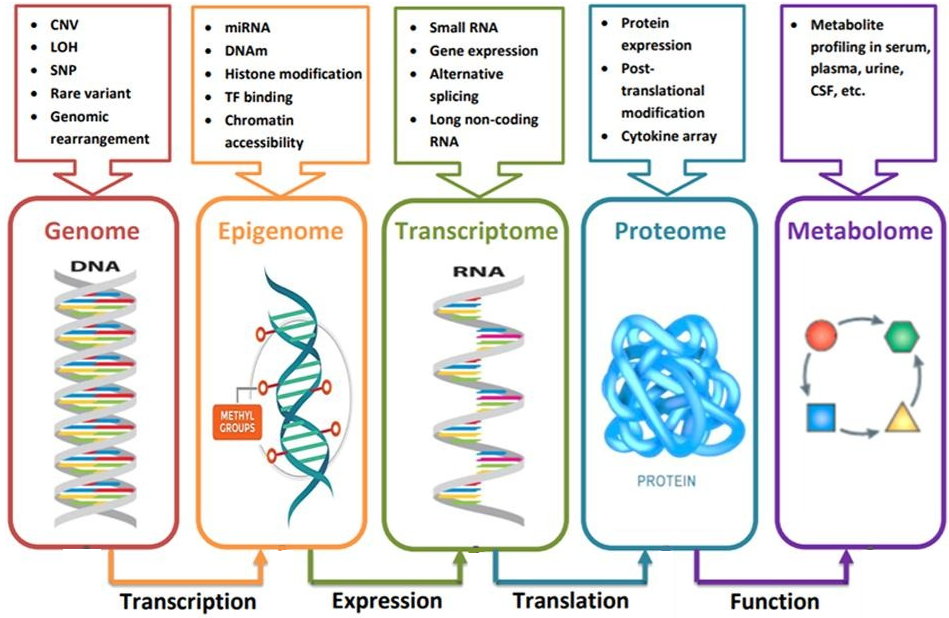
\includegraphics[width=1\textwidth]{figures/intro_omics.png}
 \caption[Méthodes de séquençages "omiques"]{Schéma des différentes méthodes de séquençages "omiques" donnant accès à une vue globale des mécanismes biologiques dans les tissus biologiques. (Modifié de \cite{momeni_survey_2020})}
 \label{fig:intro-omics}
\end{figure}
Les données de séquençages sont massives, le génome humain mesurant environ 3,1~milliards de paires de bases (bp), le séquençage d'un génome unique avec une profondeur de 50X (nécessaire pour la détection de mutation génétique) représente un minimum de 150~milliards de paires de bases lues et stockées, pour un individu. Ces données de séquence massives requièrent des outils spécifiques et un matériel informatique adapté à leur traitement. De plus la détection de mutations pathogène est complexe. L'identification du gène responsable d'une maladie génétique reste un challenge lors du diagnostic, même avec les données de séquençage complètes.

La collecte et l'intégration de l'ensemble de ces données biomédicales générées grâce aux nouvelles technologies haut débit en imagerie, séquençage et \gls{dse} ont le potentiel d'améliorer la compréhension des maladies et la prise en charge des patients.

\subsection{Collecte et utilisation des données biomédicales au service du patient}
Le Royaume-Uni est un pays pionnier dans la collecte et la mise à disposition de façon massive de données biomédicales à travers le \gls{nhs}. Cela s'illustre par exemple par le projet "100 000 génomes" lancé en 2012 qui a pour but de séquencer 100 000 génomes de patient anglais pour améliorer la recherche et le diagnostic de maladie rares, certains cancers et maladies infectieuses (\cite{nunn_public_2019}). En avril 2022 a été publié le rapport de 112 pages intitulé: "\textit{Better, broader, safer: using health data for research and analysis}" (\cite{ben_goldacre_better_2022}), écrit par le professeur Ben Goldacre missionné par le \gls{nhs}. Ce rapport met en évidence le challenge et la stratégie à adopter pour une collecte et un usage à grande échelle de données biomédicales de patients. Le projet OpenSAFELY (\href{https://www.opensafely.org/}{https://www.opensafely.org/}), fondé par Ben Goldacre, est un exemple concret d'utilisation de données biomédicales au service de la recherche et de la prise en charge de patients. Ce projet, créé en juin 2020 pour lutter contre la pandémie de COVID-19, met à disposition des chercheurs des outils et des données biomédicales massives de patients. À ce jour, ce projet a permis la publication des plus de 80 publications scientifiques de recherches réalisées à partir de ces données. Des initiatives similaires  mettent en évidence l'utilité des big data biomédicales comme catalyseur de découvertes scientifiques, telles que le projet "Big Data to Knowledge" fondé par le \textit{National Institutes of Health (NIH)} (\cite{toga_big_2015}).

Outre la phase de collecte, la difficulté dans l'exploitation des données biomédicale réside dans la disponibilité de techniques d'analyse adaptées (\cite{wang_big_2019, ismail_requirements_2020}). Les données biomédicales étant volumineuses, complexes et multimodales, leurs explorations manuelles ou via des techniques statistiques de base ne sont pas suffisantes. Une des solutions à l'exploitation des données biomédicales réside dans l'utilisation de l'intelligence artificielle, et plus spécifiquement de la branche nommée \gls{ml} pour construire des systèmes capables d'exploiter ces données.

\section{Machine-Learning pour le traitement des données biomédicales}
Le \textit{machine-learning} est une branche de l'\gls{ia} qui regroupe un ensemble d'algorithmes capables d'accomplir une tâche en apprenant d'un jeu de données. Dans cette section, nous allons définir les concepts des bases du \gls{ml} tel que le format des données, les tâches qui peuvent être accomplies, les méthodes d'apprentissages et les principaux algorithmes utilisés.

\subsection{Les formats et partitionnements des données}
Les données sont le point fondamental et critique des techniques de \gls{ml}. Les données représentent l'ensemble des informations brutes utilisées par notre algorithme de \gls{ml} pour réaliser son apprentissage et réaliser des prédictions. Pour être utilisables par les algorithmes de \gls{ml} les données doivent être structurées. Le tableau \ref{table:dataset_intro} présente un exemple de structure d'un jeu de données exploitable pour un algorithme de \gls{ml}. Les données sont sous la forme de tableau où chaque ligne représente une observation (un point de données, par exemple un patient) et chaque colonne représente un descripteur (nommé \textit{feature} en anglais, par exemple le rythme cardiaque, la présence d'une toux chez le patient, la présence d'antécédents de diabète...). Enfin la dernière colonne représente le label, c'est en général ce que l'on souhaite prédire dans le cadre de l'entrainement de notre modèle.
\begin{table}[h!]
\centering
\begin{tabular}{|c|c|c|c|c|} 
 \hline
 ID Patient & Rythme Cardiaque (bpm) & Toux & Diabiète & Diagnostic \\
 \hline
 1 & 86 & non & non & Sain \\ 
 2 & 65 & non & non & Sain \\ 
 3 & 59 & non & non & Sain \\ 
 4 & 95 & oui & non & Malade \\ 
 5 & 101 & oui & oui & Malade\\ 
 \hline
\end{tabular}
\caption{Exemple de tableau de données fictives de patients}
\label{table:dataset_intro}
\end{table}
Cette contrainte sur la structure nécessaire du jeu de données pour les algorithmes de \gls{ml} mets en évidence les limites de leurs utilisations pour l'analyse de données non structurées telles que le texte libre, les données d'imageries ou les données de séquence d'ADN. Il est nécessaire en amont de structurer ces données à travers des descripteurs pertinents pour les exploiter.

De plus, il est nécessaire de partitionner ce jeu de données sous forme de tableau en deux: les données d'apprentissage et les données de test. Les données d'apprentissage sont les données qui vont être utilisées par l'algorithme de \gls{ml} pour réaliser son entrainement, c'est-à-dire pour apprendre à réaliser la tâche définie (prédiction du label par exemple). Le jeu de test quant à lui contient des données qui n'ont jamais été présentées au modèle au cours de l'apprentissage. Le modèle entrainé va alors prédire le label du jeu de test et les prédictions réalisées sont comparées aux labels réels. Cela permet d'évaluer les performances de notre entrainement. Pour donner un ordre de grandeur, il est commun d'utiliser 80\% des données comme jeu d'entrainement et 20\% des données restantes comme jeu de test.

Pour finir, il existe un troisième partitionnement des données optionnel nommé jeu de validation. Le jeu de validation est réalisé en général en prenant 10\% des données d'entrainement. Ce jeu de validation permet d'évaluer le modèle au cours de l'entrainement et  ajuster ses paramètres. Ceci permet de s'assurer que l'entrainement progresse correctement avant de tester les performances à la fin de l'entrainement sur le jeu de test.

\subsection{Les différentes tâches que le machine-learning peut accomplir}
Les algorithmes de \gls{ml} peuvent accomplir de multiples tâches dont quatre principales. Il y a: (i) les algorithmes de classifications (ii) de régression (iii) de clustering et (iv) de réduction de dimensionnalité.

Les tâches de classification sont les plus communes. Il s'agit ici d'apprendre à prédire une classe ou un label pour un point de donnée. Par exemple il peut s'agir dans le cadre de données biomédicales de la prédiction d'un diagnostic parmi une liste de maladies. Cette classification peut-être binaire (2 classes uniquement, par exemple sain vs malade) ou multiclasse (plus de 2 classes, par exemple faire la différence entre 10 diagnostics possibles). Enfin cette classification peut aussi être multilabel, c'est-à-dire que l'on peut prédire plusieurs classes pour un point de donnée. Par exemple, si l’on construit un algorithme capable de prédire le genre d'un film de cinéma, il est utile d'avoir un système de classification multilabel pour prédire plusieurs genres (comédie et horreur par exemple) pour un même film. Parmi les algorithmes de \gls{ml} capables de faire de la classification, on retrouve de nombreux outils tels que les méthodes bayésiennes, les méthodes à bases d'arbres (arbre de décision, forêt aléatoire), les régressions logistiques où encore les systèmes de classeurs.

Les tâches de régressions ne cherchent pas à prédire une catégorie, mais une valeur numérique. Par exemple, on peut construire un modèle \gls{ml} capable de prédire le prix d'une maison ou encore la pression sanguine d'un patient, dans ces cas-là on cherche à prédire une valeur numérique continue. Les algorithmes à base d'arbres sont aussi capables de réaliser des tâches de régressions (arbre de décisions, forêt aléatoire) et on retrouve aussi d'autres algorithmes tels que la régression Lasso, Ridge et régression linéaire, qui est l'algorithme de base pour les taches de régression.

Les tâches de clustering cherchent à regrouper les points de données similaires en sous-groupes, c'est-à-dire en cluster. Les techniques de clustering sont utilisées dans le domaine biomédical pour analyser les données d'expression génétique. À partir de l'expression des gènes d'une cohorte de patients, il est possible d'utiliser des algorithmes de clustering pour trouver des sous-groupes de patients ayant un profil génétique similaire par exemple dans le cadre d'une comparaison de l'expression des gènes chez des patients sains et des patients atteints de cancer. Les algorithmes classiques de clustering sont l'algorithme K-means, DBSCAN et le clustering hiérarchique.

Pour finir, les tâches de réduction de dimensionnalité consistent à réduire le nombre de variables aléatoires d'un jeu de données en obtenant un ensemble de variables principales. Typiquement, les données à haute dimensionnalité comme les données transcriptomiques (expression de plusieurs dizaines de milliers d'ARN) sont complexes à analyser et présentent des problèmes spécifiques à cette haute dimensionnalité, connus sous le nom de la malédiction de la dimension (\textit{curse of dimensionality}). Les techniques de réduction de dimensionnalité tendent à atténuer ce problème. Les algorithmes de réduction de dimensionnalités sont typiquement utilisés après une étape de clustering pour observer graphiquement les clusters obtenus en un graphique 2D. Pour reprendre l'exemple précédant, après une analyse transcriptomique, une étape de réduction de dimensionnalité peut-être appliquée pour visualiser quel est le principal axe de différenciations de nos échantillons. Les algorithmes de réductions de dimensionnalité communément utilisés sont la PCA, le t-SNE et UMAP.

\subsection{Apprentissage supervisé, non supervisé et par renforcement}
Les différentes tâches présentées peuvent se regrouper sous trois méthodes d'apprentissages différentes: l'apprentissage supervisé, non supervisé et par renforcement.

Les tâches de classification et de régression sont possibles grâce à l'apprentissage supervisé. En apprentissage supervisé le modèle est entrainé sur des données labellisées, c'est-à-dire des données pour lesquels on connait déjà le résultat attendu (diagnostic par exemple). Ainsi le modèle est entrainé à reproduire ces labels automatiquement.
Les taches de clustering et de réduction de dimensionnalités sont possibles grâce à l'apprentissage non supervisé. En apprentissage non supervisé, les labels des données ne sont pas connus. L'objectif est donc de découvrir le structure cachée des données à partir des descripteurs. Ainsi le modèle essaie de déterminer des groupes ou des regroupements de dimensions qu'il détermine comme pertinents, mais sans connaitre le résultat réel attendu.

Enfin l'apprentissage par renforcement est moins connu et représente une méthode d'apprentissage où un agent (modèle) apprend à se comporter dans un environnement donné, recevant des pénalités et des récompenses en fonction de ses actions. Typiquement,  un modèle apprenant à jouer à un jeu d'échecs représente une tâche d'apprentissage par renforcement. Dans un cadre biomédical, un système d'apprentissage par renforcement peut être utile par exemple pour un système d'examen médical intelligent qui va proposer des symptômes à vérifier chez le patient en fonction des observations déjà enregistrées. Ainsi on a un environnement (les observations réalisées chez le patient) et des actions à réaliser par le modèle de \gls{ml} (proposer des symptômes ou examens à vérifier). Les algorithmes utilisés pour ce type d'apprentissage peuvent être des réseaux de neurones, les méthodes de \textit{Q-learning} ou encore les systèmes de classeurs.

La figure \ref{fig:ml-landscape} représente schématiquement la classification des tâches, des modes d'apprentissages et des différents cas d'applications et algorithmes associés.
\begin{figure}[!htbp]
 \centering
 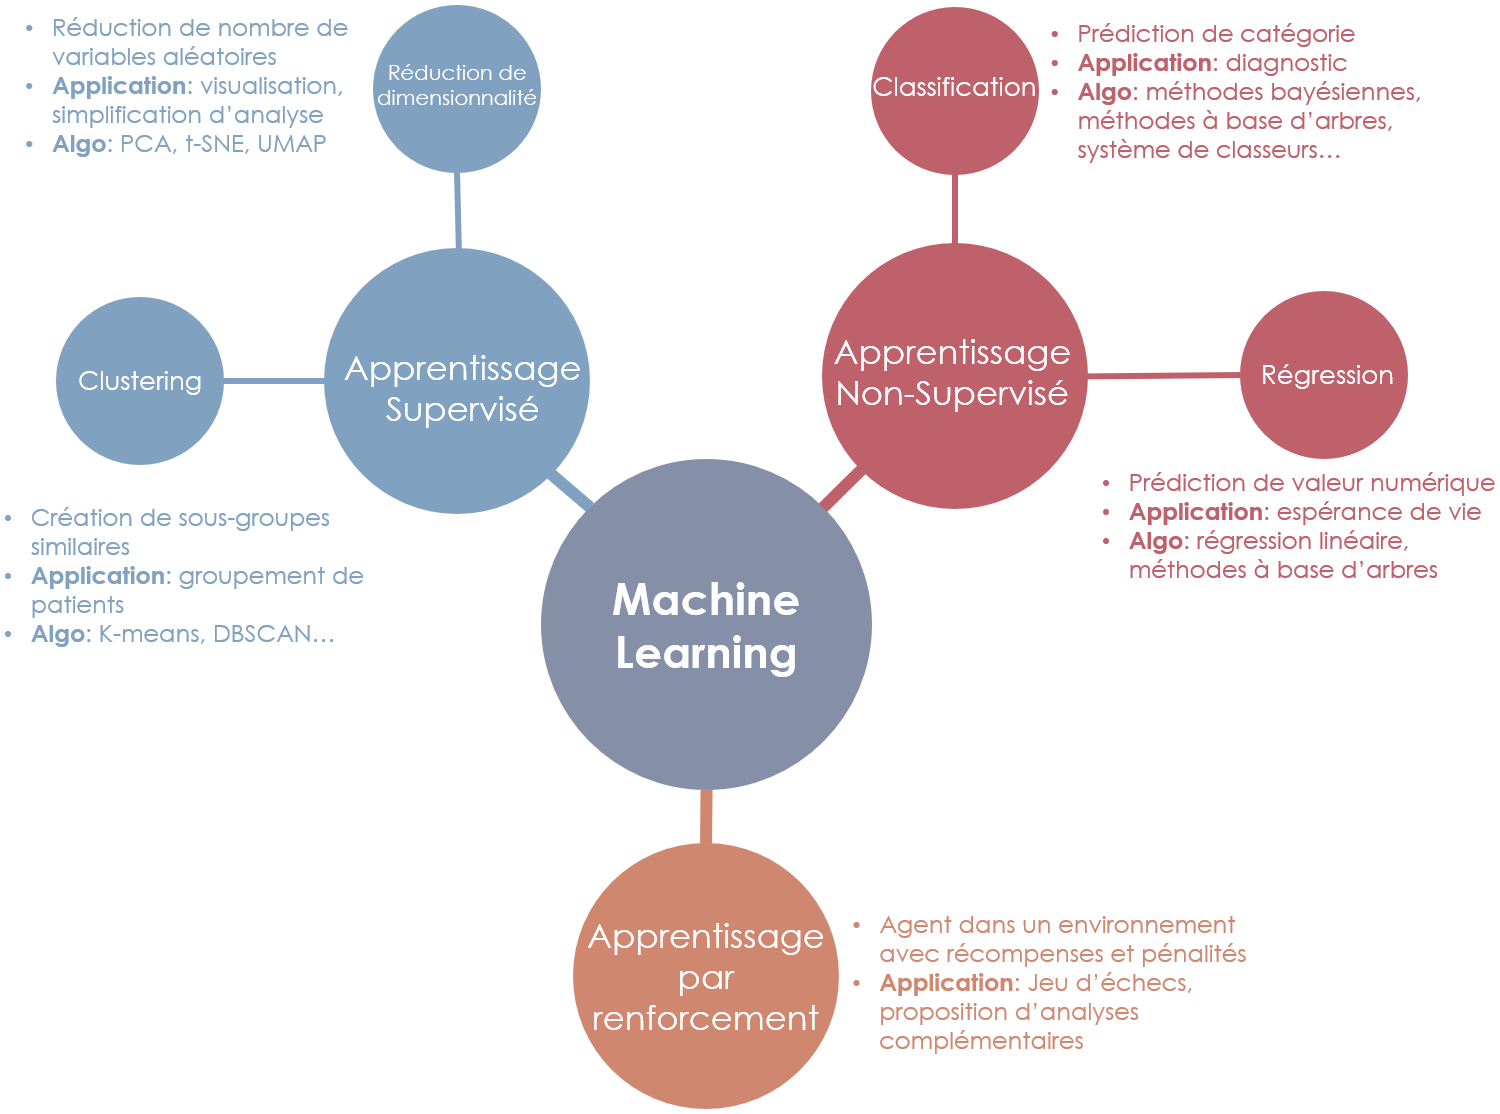
\includegraphics[width=1\textwidth]{figures/ml_landscape.png}
 \caption[Schéma des méthodes de machine-learning]{Schéma de la classification des tâches, des modes d'apprentissage et des différents cas d'applications et algorithmes associés en \textit{machine-learning}}
 \label{fig:ml-landscape}
\end{figure}

\subsection{Algorithmes de \textit{machine-learning} et explicabilité}
Enfin, dans cette section de présentation des outils de \gls{ml}, nous allons présenter la notion d'explicabilité des algorithmes de \gls{ml} et son importance dans le domaine biomédicale. Ainsi nous allons voir quelques exemples d'algorithmes de \gls{ml} couramment utilisés pour voir leur fonctionnement et leur niveau d'explicabilité.

\subsubsection{Le concept d'explicabilité}
D'après l'essai philosophique "\textit{Studies in the logic of explanation}" de Carl G. Hempel et Paul Oppenheim en 1948 (\cite{hempel_studies_1948}), le concept d'explication scientifique peut se résumé en une équation:
\[\sum C + \sum L = E\]
Dans cette équation, C représente l'ensemble des conditions antérieures et L représente l'ensemble des lois générales. La somme des conditions et des lois permet de produire E, l'évènement ou le phénomène observé. Les termes de gauche représentent ce qu’on nomme l’\textit{explanans} (l’expliquant) et le terme de droite est référé comme l’\textit{explanandum} (l’explicable). L’équation mathématique implique que l’on peut la lire dans les deux sens. C’est-à-dire qu’en connaissant E (le phénomène) nous pouvons déduire C et L (les conditions et lois) nous réalisons donc une explication scientifique. À l’inverse, en connaissant C et L (les conditions et lois) nous pouvons déduire E (le phénomène), nous faisons alors une prédiction. Optimalement, une explication est adéquate si l’\textit{explanans} permet de prédire totalement le phénomène observé.

Appliqué au \textit{machine-learning}, C représente alors les points de données et leurs descripteurs (conditions initiales), L représente notre modèle de \gls{ml} et ses règles internes tandis que E représente la prédiction du modèle.

Les récentes recherches en \gls{ia} ont amené à l'émergence du domaine d'\gls{xai}. L'\gls{xai} cherche à concevoir des méthodes pour rendre les modèles d'\gls{ia} et de \gls{ml} plus transparents et explicables, ce qui est critique dans le cadre de l'application de ces modèles dans des domaines à haut risque, comme le domaine médical (\cite{arrieta_explainable_2019}). C'est-à-dire concevoir des méthodes de \gls{ml} dont on est capable de comprendre et d'évaluer les prédictions de manière intelligible.

La figure (\ref{fig:xai-research}) présente le concept de compromis entre performances des algorithmes et leur niveau d'explicabilité. De manière générale, plus un algorithme est performant d'un point de vue prédictif, moins il est explicable. Le domaine de l'\gls{xai} cherche donc a soit: (i) améliorer l'explicabilité des algorithmes performants et peu explicables ou (ii) améliorer les performances des modèles les plus explicables.
\begin{figure}[!htbp]
 \centering
 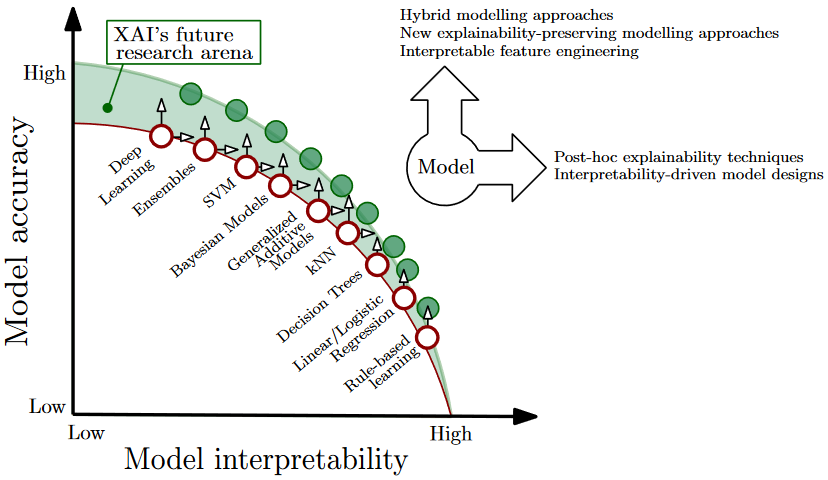
\includegraphics[width=1\textwidth]{figures/xai-research.png}
 \caption[Compromis entre interprétabilité et performances des algo de ML]{Compromis entre interprétabilité du modèle et performance d'algorithmes de ML. Représentation de la zone d'amélioration où réside le potentiel des techniques et outils de l'IA explicable (xAI) (Source: \cite{arrieta_explainable_2019})}
 \label{fig:xai-research}
\end{figure}

Au regard de l'explicabilité d'un modèle, en \gls{ml}, il y a deux catégories d'algorithmes: (i) les algorithmes transparents par design, c'est-à-dire directement explicables et (ii) les algorithmes sous forme de boites noires, dont l'explicabilité n'est accessible que grâce à des méthodes \textit{post-hoc}. Dans les prochaines sous-sections, nous allons présenter le fonctionnement de quelques algorithmes de façon non exhaustifs pour chaque catégorie. Nous allons ainsi voir les méthodes bayésiennes, les arbres de décisions et les systèmes de classeurs comme méthodes transparents. Puis les méthodes de forêts aléatoires et de boosting comme méthodes à explicabilité post-hoc.

\subsubsection{Méthodes bayésiennes}
Les méthodes bayésiennes naïves reposent sur le théorème de Bayes sur les probabilités conditionnelles avec une hypothèse d'indépendance forte (c'est-à-dire naïve) entre les descripteurs. Pour chaque descripteur, la probabilité d'une classe est calculée en fonction de la valeur du descripteur. Grâce à cette caractéristique probabiliste, le modèle est capable de fournir une prédiction et une mesure de l'incertitude associée. Les méthodes bayésiennes sont transparentes, car il est facile de décomposer la contribution de chaque descripteur lors d'une prédiction.

\subsubsection{Méthodes à base d'arbres}
Les arbres de décisions sont des modèles classiques en \gls{ml}. Cette méthode cherche à produire un arbre (un graphe dirigé acyclique) où chaque nœud s'apparente à une série de questions posée sur les descripteurs des données. En fonction de la valeur de ces descripteurs, l'arbre progresse vers un sous-nœud jusqu'à la prédiction, le nœud feuille final. Cette méthode est intrinsèquement explicable, car il est facile de dessiner l'arbre et de retracer le processus de prédiction pour un point de données en suivant les nœuds comme une série de règles logiques. Par exemple la figure \ref{fig:decision-tree} présente un exemple d'arbre de décisions très simple avec trois nœuds (3 questions pour 3 descripteurs) et deux classes possibles comme prédiction (nœud feuille final rond).
\begin{figure}[!htbp]
 \centering
 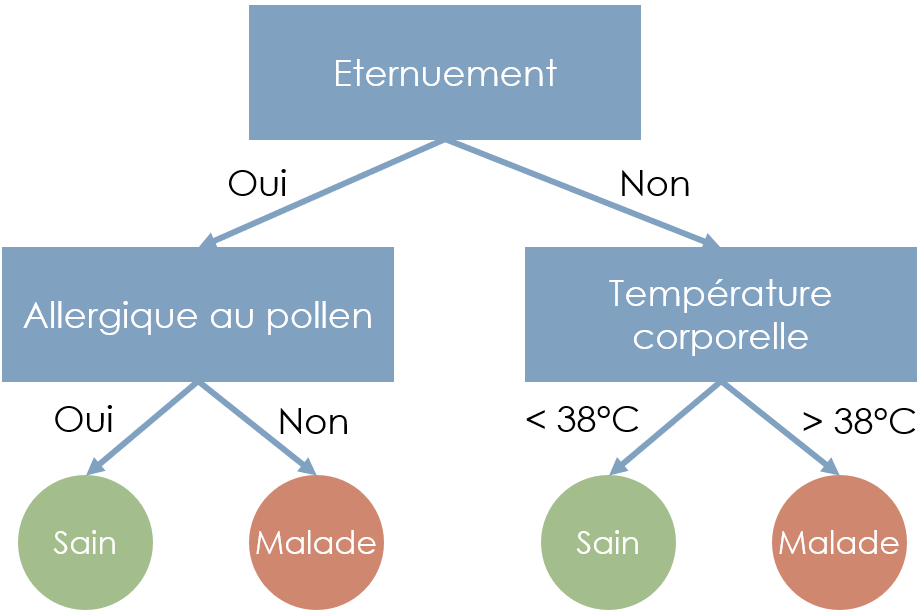
\includegraphics[width=0.6\textwidth]{figures/decision_tree.png}
 \caption[Exemple d'arbre de décision]{Exemple d'arbre de décision à 3 questions (3 nœuds pour 3 descripteurs) et 2 classes.}
 \label{fig:decision-tree}
\end{figure}

Une évolution des arbres de décisions pour les rendre plus complexes et performants est nommée la méthode de la forêt aléatoire qui est une méthode ensembliste des arbres de décision. La figure \ref{fig:random-forest} présente le fonctionnement de la forêt aléatoire. Cela consiste à construire plusieurs arbres de décisions sur des sous-ensembles de nos données, puis de combiner les prédictions de ces arbres. Chaque arbre de décisions ainsi généré va établir une prédiction et la prédiction finale correspondra à la majorité des votes de chaque arbre. Les méthodes de \textit{boosting}  (XGBoost, LGBoost, CatBoost) sont similaires aux forêts aléatoires à la différence que chaque arbre n'est pas construites indépendamment, mais il cherche à corriger les erreurs du précédent, de manière séquentielle.
\begin{figure}[!htbp]
 \centering
 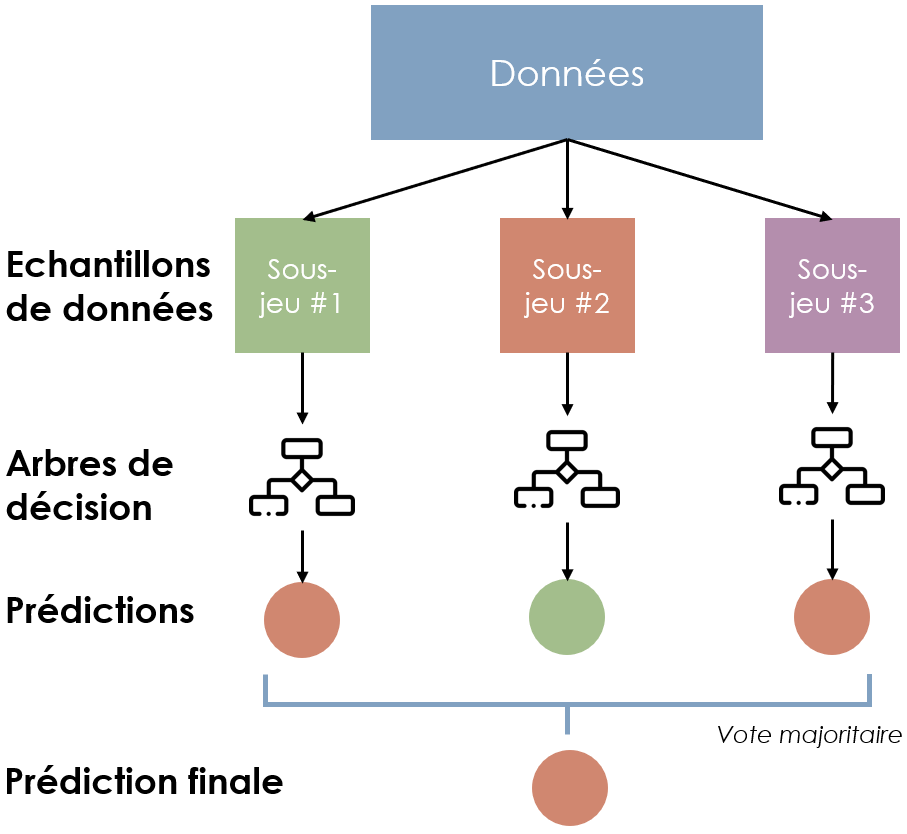
\includegraphics[width=0.7\textwidth]{figures/random_forest.png}
 \caption[Fonctionnement de l'algorithme de forêt aléatoire]{Fonctionnement de l'algorithme de forêt aléatoire}
 \label{fig:random-forest}
\end{figure}
Les forêts aléatoires sont très utilisées en \gls{ml} et spécifique en biologie. En exemple d'application dans le domaine biomédicale, l'outil MISTIC (\textit{MISsense deleTeriousness predICtor}, \cite{chennen_mistic_2020}) développé dans notre équipe utilise des méthodes de forêts aléatoires pour calculer la pathogénicité des variants génétiques. Cependant, la forêt aléatoire et les méthodes de boosting perdent en explicabilité. En effet, en raison du grand nombre d'arbres de décision générés, il n'est plus possible de suivre aisément le processus de prédiction suivant une suite de règles logique pour un point de donnée. Il faut alors utiliser des méthodes d'explicabilité \textit{ad-hoc} qui consistent à calculer l'importance numérique de chaque descripteur pour une prédiction donnée.

\subsubsection{Systèmes de classeurs (LCS)}
Les \gls{lcs} sont des algorithmes de \gls{ml} les plus transparents et explicables (figure \ref{fig:xai-research}, \cite{arrieta_explainable_2019}). Ces systèmes fonctionnent sur le principe d'un ensemble de règles (nommées "classeurs"), qui associent des conditions à une action (prédiction). La table \ref{table:lcs-rules} présente un exemple de trois règles fictives issues de l'entrainement d'un \gls{lcs}. Une règle (ou un classeur) se présente sous la forme "SI [condition] ALORS [prédiction]". Chaque règle est associée à un poids, ce qui permet de définir une importance plus ou moins forte. Leur fonctionnement est donc similaire aux arbres de décisions, mais sans sens imposés entre les séries de questions.
\begin{table}[!htbp]
\centering
\begin{tabular}{|l|l|c|} 
 \hline
 Conditions & Prédiction & Poids \\
 \hline
 SI éternuement ET allergique au pollen & ALORS sain & 7 \\ 
 SI temp. corporelle > 38°C & ALORS malade & 12  \\ 
 SI éternuement ET temp. corporelle = 37°C & ALORS sain & 3  \\ 

 \hline
\end{tabular}
\caption{Exemple de règles fictives issues de l'entrainement d'un algorithme de LCS}
\label{table:lcs-rules}
\end{table}

L'apprentissage des systèmes de classeurs se réalise par des mécanismes d'évolutions. Chaque règle va être initialement générée de façon aléatoire (ou guidée, \cite{urbanowicz_relief-based_2018}) puis modifiée aléatoirement (mutée) au fur et à mesure des cycles d'entrainement (génération). A chaque cycle, les règles les moins performantes lors de l'évaluation sur le jeu d'entrainement sont éliminées du jeu de règles. Ainsi au bout d'un certain nombre de cycles (générations), les règles générées qui ont survécu au processus de sélections sont performantes dans leurs taches de classification.

Les \gls{lcs} sont extrêmement explicables, car leur apprentissage génère une liste de règles parfaitement intelligible pour l'Homme, ainsi il est facile de reproduire le processus de prédiction des points de données manuellement (\cite{arrieta_explainable_2019}). Aussi, pour chaque prédiction, il est possible de savoir exactement quelles sont les règles qui ont été déclenchées et qui ont mené à cette prédiction. Cependant ces systèmes restent sous-performants et leurs méthodes d'apprentissage par évolution posent des difficultés de mise à l'échelle et nécessitent un grand nombre de données pour être efficaces (\cite{urbanowicz_exstracs_2015}).

\subsection{Limites du \textit{machine-learning} appliqué aux données biomédicales}
Bien que les techniques de \gls{ml} se révèlent utiles pour traiter, analyse et prédire de grands ensembles de données, ces techniques font face à de grandes difficultés dans le cadre des données biomédicales (\cite{martinez-garcia_data_2022}). Les données biomédicales étant massives, mais surtout non structurées et multimodales, il est difficile de réaliser le travail d'annotation nécessaire à leurs structurations pour l'utilisation d'algorithme de \gls{ml}. Car l'annotation manuelle des données est un travail couteux en temps et en argent, d'autant plus dans le domaine médical ou l'annotateur doit être un expert du domaine. Ainsi il est nécessaire de développer des méthodes d'\gls{ia} capables d'apprendre et d'exploiter les données brutes non structurées sous toutes les formes (textes, images, séquences).

Dans ce contexte-là, les réseaux de neurones profonds présentent une opportunité pour le traitement des données biomédicales non structurée. En effet, les réseaux de neurones sont parmi les modèles les plus performants et sont capables de traiter aisément des données non structurées en extrayant eux-mêmes les descripteurs pertinents à partir de la structure des données. Cependant ce sont aussi de complètes boites noires et non explicables. Dans le prochain chapitre, nous verrons comment les réseaux de neurones profonds fonctionnent et peuvent être utilisés pour traiter les données biomédicales non structurées là où les techniques de \gls{ml} classique échouent.